\documentclass[11pt]{report}
\usepackage[utf8]{inputenc}
\usepackage{babel}
\babelprovide[main,import]{spanish}
\usepackage{amsmath,amssymb,amsthm}
\usepackage{geometry}
\geometry{margin=2.4cm}
\usepackage{setspace}
\onehalfspacing
\usepackage{booktabs}
\usepackage{graphicx}
\usepackage{tikz}
\usepackage{pgfplots}
\pgfplotsset{compat=1.18}
\usepackage{hyperref}
\renewcommand{\thesection}{\arabic{section}}
\newcommand{\ket}[1]{\left|#1\right\rangle}
\newcommand{\bra}[1]{\left\langle#1\right|}
\newcommand{\spl}{\sigma_{+}}
\newcommand{\smi}{\sigma_{-}}
\newcommand{\Pe}{\ket{e}\!\bra{e}}
\newcommand{\Pg}{\ket{g}\!\bra{g}}
\newcommand{\D}{\mathcal{D}}
\newcommand{\Lv}{\mathcal{L}}

\title{Qubits gato estabilizados por un qubit con acoplamientos transversal y longitudinal:\\ teor\'ia completa, verificaci\'on num\'erica y reglas de dise\~no\\[1ex] \large Documento de trabajo, versi\'on 1}
\author{Jhon Sebasti\'an Garc\'ia Barrera}
\date{Septiembre de 2026}

\begin{document}
\maketitle
\tableofcontents

%======================================================================
\section{Prop\'osito y alcance del documento}

Este documento re\'une toda la teor\'ia, las derivaciones, los resultados num\'ericos y las figuras producidas hasta ahora. No es el art\'iculo: es el registro completo del cual se extraer\'a. Por eso incluye tambi\'en los resultados que se corrigieron o retiraron durante el trabajo, con la raz\'on de cada cambio.

La pregunta central es la siguiente. Existe una familia de esquemas en los que un qubit con acoplamiento transversal $g_{x}$ y longitudinal $g_{z}$ a un oscilador de frecuencia $\omega$, con el qubit a frecuencia cercana a $2\omega$ y excitado por un drive, estabiliza un estado gato en el oscilador mediante disipaci\'on de pares. La familia incluye el esquema de microondas de Ma, Xie y Li \cite{Ma2019}, el mec\'anico de Naseem \cite{Naseem2026} y los magn\'onicos de Hou et al.\ \cite{Hou2024} y Liu et al.\ \cite{Liu2025}. Todos esos trabajos estudian la preparaci\'on del estado. Aqu\'i se estudia el desempe\~no del estado como qubit l\'ogico: qu\'e condiciones de operaci\'on requiere, qu\'e fija la tasa de errores de fase, c\'omo se puede mejorar, qu\'e limita el confinamiento y qu\'e exige la temperatura.

Los resultados principales son cuatro reglas v\'alidas para toda la familia:
\begin{enumerate}
\item La condici\'on de operaci\'on: el drive debe sintonizarse al doble de la frecuencia vestida del oscilador, $\omega_{p}^{*}=2(\omega-4g_{x}^{2}/3\omega)$, con una tolerancia del orden de $3G$, donde $G=2g_{x}g_{z}/\omega$.
\item La figura de m\'erito: $\kappa_{1}/\kappa_{2}=(5/72)(\kappa/g_{z})^{2}$, independiente de $g_{x}$ y de $\omega$, con su generalizaci\'on a un baño estructurado.
\item El techo del confinamiento, que satura en el orden de $\kappa/4$ por ser el auxiliar un sistema de dos niveles.
\item El requisito t\'ermico: $hf_{q}/k_{B}T\gtrsim9$ para un sesgo de 100 con $|\alpha|^{2}=2$.
\end{enumerate}

%======================================================================
\section{Modelo y convenciones}

\subsection{Hamiltoniano y ecuaci\'on maestra}

El modelo com\'un a la familia es
\begin{equation}
H(t)=\omega a^{\dagger}a+\frac{\omega_{q}}{2}\sigma_{z}+(a+a^{\dagger})\left(g_{x}\sigma_{x}+g_{z}\sigma_{z}\right)+\Omega\left(\spl e^{-i\omega_{p}t}+\smi e^{i\omega_{p}t}\right),
\label{eq:H}
\end{equation}
con $\sigma_{z}=\Pe-\Pg$, $\sigma_{x}=\spl+\smi$, $\spl=\ket{e}\bra{g}$ y $\smi=\ket{g}\bra{e}$. La din\'amica es
\begin{equation}
\dot\rho=-i[H(t),\rho]+\kappa\,\D[\smi]\rho+\gamma\,\D[a]\rho,\qquad \D[L]\rho=L\rho L^{\dagger}-\tfrac{1}{2}\{L^{\dagger}L,\rho\}.
\label{eq:ME}
\end{equation}
Con temperatura se agregan los disipadores $\kappa n_{q}\D[\spl]$ en el qubit y $\gamma n_{m}\D[a^{\dagger}]$ en el oscilador (Secci\'on~\ref{sec:termico}).

\subsection{Unidades y par\'ametros de referencia}

Las frecuencias se expresan como frecuencias angulares en unidades de $2\pi\times$GHz (o $2\pi\times$MHz cuando se indica). Los tres conjuntos de par\'ametros usados son:

\begin{table}[h]
\centering
\begin{tabular}{lccc}
\toprule
 & Ma et al.\ \cite{Ma2019} & Naseem \cite{Naseem2026} & Liu et al.\ \cite{Liu2025}\\
\midrule
$\omega/2\pi$ & 6 GHz & 100 MHz & 17.7 MHz ($\nu/2$)\\
$g_{x}$, $g_{z}$ ($/2\pi$) & $-212$, $212$ MHz & 0.6, 6 MHz & 3.54, 3.54 MHz\\
$\kappa/2\pi$ & 30 MHz & 100 kHz & 16 MHz\\
$\Omega$ o $\varepsilon$ & $\Omega/2\pi=60$ MHz & $\varepsilon=4g$ & $\varepsilon_{p}/2\pi=3.53$ MHz\\
$\omega_{q}$ & $12$ GHz & $200$ MHz & (qubit vestido, $\nu=35.4$ MHz)\\
\bottomrule
\end{tabular}
\caption{Par\'ametros publicados. En Ma et al.\ el disipador es $\Gamma[2\smi\rho\spl-\spl\smi\rho-\rho\spl\smi]$ con $\Gamma/2\pi=15$ MHz, lo que equivale a $\kappa=2\Gamma$; su $g_{x}=-g\sin\theta$ y $g_{z}=g\cos\theta$ con $g/2\pi=0.3$ GHz y $\theta=\pi/4$.}
\end{table}

%======================================================================
\section{Teor\'ia efectiva de segundo orden}

\subsection{Imagen de interacci\'on}

Se toma $H_{0}=\omega a^{\dagger}a+(\omega_{q}/2)\sigma_{z}$ con $\omega_{q}=2\omega$. Con $U_{0}=e^{iH_{0}t}$,
\begin{equation}
a\to a e^{-i\omega t},\quad a^{\dagger}\to a^{\dagger}e^{i\omega t},\quad \smi\to\smi e^{-2i\omega t},\quad \spl\to\spl e^{2i\omega t},\quad \sigma_{z}\to\sigma_{z}.
\end{equation}
El acoplamiento transversal se descompone en
\begin{align}
g_{x}(\spl+\smi)(a+a^{\dagger})\;\to\;&g_{x}\left[\spl a\,e^{i\omega t}+\smi a^{\dagger}e^{-i\omega t}\right]+g_{x}\left[\spl a^{\dagger}e^{3i\omega t}+\smi a\,e^{-3i\omega t}\right],
\end{align}
donde el primer corchete es el rotante (frecuencia $\omega$) y el segundo el contrarrotante (frecuencia $3\omega$). El longitudinal da $g_{z}\sigma_{z}(ae^{-i\omega t}+a^{\dagger}e^{i\omega t})$.

\subsection{F\'ormula de James y Jerke}

Si $H_{I}(t)=\sum_{n}(h_{n}e^{-i\omega_{n}t}+h_{n}^{\dagger}e^{i\omega_{n}t})$, con $\omega_{n}>0$ grandes frente a los acoplamientos, el Hamiltoniano efectivo promediado es \cite{JamesJerke2007}
\begin{equation}
H_{\rm ef}=\sum_{m,n}\frac{1}{\bar\omega_{mn}}[h_{m}^{\dagger},h_{n}]e^{i(\omega_{m}-\omega_{n})t},\qquad \frac{1}{\bar\omega_{mn}}=\frac{1}{2}\left(\frac{1}{\omega_{m}}+\frac{1}{\omega_{n}}\right),
\end{equation}
conservando solo los t\'erminos con $\omega_{m}=\omega_{n}$. Aqu\'i hay dos frecuencias:
\begin{equation}
h_{1}=A+B,\quad A=g_{x}\smi a^{\dagger},\quad B=g_{z}\sigma_{z}a\quad(\text{frecuencia }\omega);\qquad h_{3}=g_{x}\smi a\quad(\text{frecuencia }3\omega).
\end{equation}
Los t\'erminos cruzados entre $h_{1}$ y $h_{3}$ oscilan a $2\omega$ y se descartan, as\'i que
\begin{equation}
H_{\rm ef}=\frac{1}{\omega}[h_{1}^{\dagger},h_{1}]+\frac{1}{3\omega}[h_{3}^{\dagger},h_{3}].
\end{equation}

\subsection{Conmutadores}

Se usan $\spl\smi=\Pe$, $\smi\spl=\Pg$, $[\sigma_{z},\spl]=2\spl$, $[\sigma_{z},\smi]=-2\smi$, $\sigma_{z}^{2}=1$, $[a,a^{\dagger}]=1$ y $n=a^{\dagger}a$.
\begin{align}
[A^{\dagger},A]&=g_{x}^{2}[\spl a,\smi a^{\dagger}]=g_{x}^{2}(\spl\smi aa^{\dagger}-\smi\spl a^{\dagger}a)=g_{x}^{2}[(n+1)\Pe-n\Pg],\\
[B^{\dagger},B]&=g_{z}^{2}\sigma_{z}^{2}(a^{\dagger}a-aa^{\dagger})=-g_{z}^{2},\\
[A^{\dagger},B]&=g_{x}g_{z}a^{2}(\spl\sigma_{z}-\sigma_{z}\spl)=-g_{x}g_{z}a^{2}[\sigma_{z},\spl]=-2g_{x}g_{z}\spl a^{2},\\
[B^{\dagger},A]&=g_{x}g_{z}a^{\dagger2}(\sigma_{z}\smi-\smi\sigma_{z})=g_{x}g_{z}a^{\dagger2}[\sigma_{z},\smi]=-2g_{x}g_{z}\smi a^{\dagger2},\\
[h_{3}^{\dagger},h_{3}]&=g_{x}^{2}[\spl a^{\dagger},\smi a]=g_{x}^{2}(\spl\smi a^{\dagger}a-\smi\spl aa^{\dagger})=g_{x}^{2}[n\Pe-(n+1)\Pg].
\end{align}

\subsection{Resultado}

Sumando y agrupando por estado del qubit:
\begin{equation}
\boxed{H_{\rm ef}=\frac{g_{x}^{2}}{\omega}\left[\left(\tfrac{4}{3}n+1\right)\Pe-\left(\tfrac{4}{3}n+\tfrac{1}{3}\right)\Pg\right]-G\left(\spl a^{2}+\smi a^{\dagger2}\right),\qquad G=\frac{2g_{x}g_{z}}{\omega}}
\label{eq:Hef}
\end{equation}
m\'as la constante $-g_{z}^{2}/\omega$. En el marco rotante del drive se agrega $\Omega(\spl+\smi)$. Tres cantidades se leen directamente:
\begin{equation}
\delta_{\rm osc}=-\frac{4g_{x}^{2}}{3\omega}\ (\text{oscilador con el qubit en }\ket{g}),\qquad +\frac{4g_{x}^{2}}{3\omega}\ (\text{en }\ket{e}),\qquad \Delta_{q}^{\rm Stark}=+\frac{4g_{x}^{2}}{3\omega}\ (\text{qubit, }n=0).
\end{equation}
De cada corrimiento, $3/4$ vienen del t\'ermino rotante y $1/4$ del contrarrotante. El corrimiento del oscilador es el corrimiento dispersivo con la correcci\'on de Bloch-Siegert, $g_{x}^{2}/\Delta+g_{x}^{2}/\Sigma$ con $\Delta=\omega_{q}-\omega=\omega$ y $\Sigma=\omega_{q}+\omega=3\omega$ \cite{Zueco2009}.

\subsection{Comparaci\'on con los trabajos previos}

\paragraph{Ma et al.} Su Ec.~(4) es $H^{\rm Ma}=(3g_{x}^{2}/\omega)\Pe+(2g_{x}^{2}/\omega)n\Pe-(2g_{x}g_{z}/\omega)(\spl a^{2}+\smi a^{\dagger2})+\Omega(\spl+\smi)$. Con solo los t\'erminos rotantes, la parte diagonal es $(g_{x}^{2}/\omega)[(n+1)\Pe-n\Pg]$, y usando $\Pg=1-\Pe$,
\begin{equation}
\frac{g_{x}^{2}}{\omega}[(n+1)\Pe-n\Pg]=\frac{g_{x}^{2}}{\omega}(2n+1)\Pe-\frac{g_{x}^{2}}{\omega}n.
\end{equation}
El primer t\'ermino reproduce su $2n\Pe$; el segundo, $-(g_{x}^{2}/\omega)n$, no aparece: es el corrimiento del oscilador con el qubit en $\ket{g}$. Su corrimiento del qubit, $3g_{x}^{2}/\omega$, no coincide con el valor exacto $4g_{x}^{2}/(3\omega)$. El coeficiente de pares s\'i es correcto.

\paragraph{Liu et al.} Su Ec.~(11) es $(8g_{x}^{2}/3\nu)(|{\uparrow}\rangle\langle{\uparrow}|+2n|{\uparrow}\rangle\langle{\uparrow}|)-g_{\rm eff}(m^{2}\tilde\sigma_{+}+{\rm h.c.})+\varepsilon_{p}(\tilde\sigma_{+}+\tilde\sigma_{-})$ con $g_{\rm eff}=4g_{x}g_{z}/\nu$. Con $\omega=\nu/2$, la parte en $\ket{e}$ es $(g_{x}^{2}/\omega)(4/3+8n/3)$, que coincide con la Ec.~\eqref{eq:Hef} reescrita con $\Pg=1-\Pe$, incluyendo los contrarrotantes; pero omite el t\'ermino $-(4g_{x}^{2}/3\omega)n$. El coeficiente de pares es correcto.

\paragraph{Naseem.} Su teor\'ia incluye un corrimiento $\delta_{1}=g_{x}^{2}[{\rm Im}\,S_{1}^{-}+{\rm Im}\,S_{1}^{+}]$ que, como se muestra en la Secci\'on~\ref{sec:RS}, es exactamente $\delta_{\rm osc}$ con una correcci\'on de orden $(\kappa/\omega)^{2}$; pero su c\'odigo num\'erico no lo incluye en el Hamiltoniano efectivo. Adem\'as, su Ec.~(11) tiene $g_{\rm eff}=g$ en lugar de $2g$, con $g=g_{x}g_{z}/\omega$.

\subsection{Verificaci\'on por diagonalizaci\'on exacta}

Se diagonaliz\'o la Ec.~\eqref{eq:H} sin drive ($\omega=1$, $\omega_{q}=2$, 30 a 46 fonones). Las tablas~\ref{tab:ED} y~\ref{tab:ED2} reúnen las dos implementaciones independientes.

\begin{table}[h]
\centering
\begin{tabular}{ccccc}
\toprule
$g_{x}$ & $g_{z}$ & oscilador en $\ket{g}$ & oscilador en $\ket{e}$ & qubit\\
\midrule
0.005 & 0 & $-1.3333$ & $+1.3332$ & $+1.3333$\\
0.01 & 0 & $-1.3332$ & $+1.3327$ & $+1.3331$\\
0.02 & 0 & $-1.3326$ & $+1.3310$ & $+1.3326$\\
0.04 & 0 & $-1.3305$ & $+1.3239$ & $+1.3303$\\
0.02 & 0.02 & $-1.3310$ & -- & --\\
0.02 & 0.04 & $-1.3262$ & -- & --\\
\midrule
\multicolumn{2}{c}{Ec.~\eqref{eq:Hef}} & $-4/3$ & $+4/3$ & $+4/3$\\
\multicolumn{2}{c}{Ma et al.} & 0 & $+2$ & $+3$\\
\bottomrule
\end{tabular}
\caption{Corrimientos en unidades de $g_{x}^{2}/\omega$. El error relativo crece como $g_{x}^{2}$: es de cuarto orden.}
\label{tab:ED}
\end{table}

\begin{table}[h]
\centering
\begin{tabular}{cccc}
\toprule
$g_{x}$ & $g_{z}$ & separaci\'on del doblete $\{\ket{g,2},\ket{e,0}\}$, exacta / $\sqrt{(4g_{x}^{2}/\omega)^{2}+8G^{2}}$ & elemento de pares / $-\sqrt2G$\\
\midrule
0.01 & 0.01 & $6.925\times10^{-4}/6.928\times10^{-4}$ & --\\
0.01 & 0.02 & -- & $0.9989$\\
$-0.01$ & 0.02 & -- & $0.9989$\\
0.02 & $-0.03$ & -- & $0.9971$\\
$-0.02$ & $-0.03$ & -- & $0.9971$\\
0.02 & 0.04 & $4.781\times10^{-3}/4.800\times10^{-3}$ & --\\
\bottomrule
\end{tabular}
\caption{Verificaci\'on independiente (V1) del bloque resonante: la separaci\'on del doblete y el signo del elemento de pares en los cuatro cuadrantes de signo de $(g_{x},g_{z})$. En el bloque, la diferencia diagonal es $4g_{x}^{2}/\omega$: $\ket{g,2}$ tiene energ\'ia $-(g_{x}^{2}/\omega)(8/3+1/3)=-3g_{x}^{2}/\omega$ y $\ket{e,0}$ tiene $+g_{x}^{2}/\omega$.}
\label{tab:ED2}
\end{table}

%======================================================================
\section{Estado oscuro y resonancia vestida}

\subsection{Marco del drive}

Se pasa al marco que rota a $\omega_{p}/2$ para el oscilador y a $\omega_{p}$ para el qubit. Con $\Delta_{m}=\omega-\omega_{p}/2$ y $\Delta_{q}=\omega_{q}-\omega_{p}$, el Hamiltoniano efectivo es
\begin{equation}
H_{\rm ef}'=\Delta_{m}n+\frac{\Delta_{q}}{2}\sigma_{z}+\frac{g_{x}^{2}}{\omega}\left[\left(\tfrac{4}{3}n+1\right)\Pe-\left(\tfrac{4}{3}n+\tfrac{1}{3}\right)\Pg\right]-G(\spl a^{2}+\smi a^{\dagger2})+\Omega(\spl+\smi).
\end{equation}

\subsection{Condici\'on de estado oscuro}

Un estado $\ket{\psi}\otimes\ket{g}$ es estacionario si lo aniquila el operador de salto, $\sqrt\kappa\smi\ket{\psi,g}=0$, lo que se cumple, y si es autoestado de $H_{\rm ef}'$. Aplicando $H_{\rm ef}'$ con $\Pe\ket{g}=0$, $\Pg\ket{g}=\ket{g}$, $\sigma_{z}\ket{g}=-\ket{g}$, $\smi\ket{g}=0$ y $\spl\ket{g}=\ket{e}$:
\begin{equation}
H_{\rm ef}'\ket{\psi,g}=\left[\left(\Delta_{m}-\tfrac{4g_{x}^{2}}{3\omega}\right)n-\tfrac{\Delta_{q}}{2}-\tfrac{g_{x}^{2}}{3\omega}\right]\ket{\psi}\otimes\ket{g}+\left(-Ga^{2}+\Omega\right)\ket{\psi}\otimes\ket{e}.
\end{equation}
Para que sea autoestado:
\begin{enumerate}
\item La componente en $\ket{e}$ debe anularse: $a^{2}\ket{\psi}=(\Omega/G)\ket{\psi}$, es decir, $\ket{\psi}\in{\rm span}\{\ket{\alpha},\ket{-\alpha}\}$ con $\alpha^{2}=\Omega/G$.
\item La componente en $\ket{g}$ debe ser proporcional a $\ket{\psi}$. Un gato no es autoestado de $n$, as\'i que el coeficiente de $n$ debe anularse: $\Delta_{m}=4g_{x}^{2}/(3\omega)$.
\end{enumerate}
La segunda condici\'on es la resonancia vestida:
\begin{equation}
\boxed{\omega_{p}^{*}=2\left(\omega-\frac{4g_{x}^{2}}{3\omega}\right)}.
\end{equation}
La desinton\'ia del qubit $\Delta_{q}$ no afecta la existencia del estado oscuro; solo cambia las tasas. Con $\omega_{p}=2\omega$ (la elecci\'on de Ma et al.) el estado oscuro no existe.

\subsection{Magnitud y verificaci\'on en el modelo completo}

Con los par\'ametros de Ma et al., $g_{x}^{2}/\omega=0.0075$ y $\delta_{\rm osc}=-0.010$ ($2\pi\times10$ MHz), un tercio de $\kappa$. Resultados del modelo completo (tres implementaciones independientes coinciden a $10^{-5}$ en $P_{c}$):

\begin{table}[h]
\centering
\begin{tabular}{lcccc}
\toprule
drive & $P_{c}$ (c\'odigo sin desplazar) & $P_{e}$ estrobosc\'opico / promedio & $|\langle a^{2}\rangle|$ & paridad final\\
\midrule
$\omega_{p}=2\omega=12$ & 0.8118 & 0.114 / 0.116 & 2.48 & 0.115 ($\Gamma t=300$)\\
$\omega_{p}=\omega_{p}^{*}=11.98$ & 0.99754 & 0.0027 / 0.0060 & 3.973 & 0.0016\\
\bottomrule
\end{tabular}
\caption{Modelo completo de Ma et al.\ en $\Gamma t=300$. $P_{c}$ es la poblaci\'on del oscilador en span$\{\ket{\pm2i}\}$. El m\'aximo del barrido fino est\'a en $\omega_{p}=11.97993$ (verificaci\'on V2), con la predicci\'on en 11.98000. La ventana con $P_{c}>0.99$ va de 11.9775 a 11.9825.}
\end{table}

\begin{figure}[h]
\centering
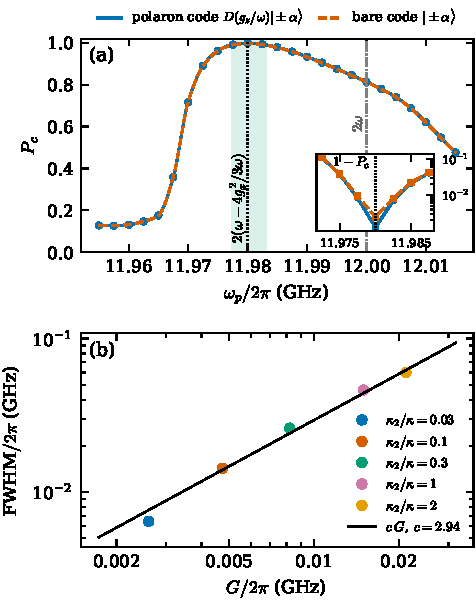
\includegraphics[width=0.62\textwidth]{fig2_val.pdf}
\caption{(a) $P_{c}$ frente a $\omega_{p}$ para el esquema de Ma et al.\ con el c\'odigo polar\'onico fijo (Secci\'on~\ref{sec:polaron}) y con el c\'odigo sin desplazar. (b) Ancho a media altura frente a $G$ para cinco valores de $\kappa_{2}/\kappa$, con el ajuste ${\rm FWHM}=cG$, $c=2.94$.}
\end{figure}

\subsection{Tolerancia: ancho de la resonancia}

El ancho a media altura de $P_{c}(\omega_{p})$ escala con $G$, no con $\kappa_{2}$:

\begin{center}
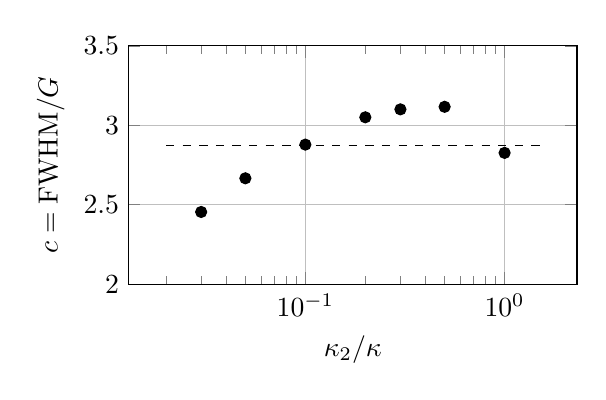
\begin{tikzpicture}
\begin{axis}[width=0.6\textwidth,height=0.38\textwidth,xmode=log,xlabel={$\kappa_{2}/\kappa$},ylabel={$c={\rm FWHM}/G$},ymin=2,ymax=3.5,grid=major]
\addplot[only marks,mark=*] coordinates {(0.03,2.454)(0.05,2.666)(0.1,2.878)(0.2,3.050)(0.3,3.100)(0.5,3.116)(1,2.826)};
\addplot[dashed,domain=0.02:1.5] {2.87};
\end{axis}
\end{tikzpicture}
\end{center}
Con siete valores de $\kappa_{2}/\kappa$ (Tarea 47(d)), $c=2.87\pm0.25$; el ajuste libre da ${\rm FWHM}\propto G^{1.10}$. En la corrida final (qubit siguiendo al drive), $c=2.94$, con rango 2.49 a 3.18. La curva es asim\'etrica: cae m\'as r\'apido hacia $\omega_{p}$ menores. La regla de dise\~no es: la frecuencia del drive debe fijarse con una precisi\'on de orden $G$; para un c\'odigo de calidad ($P_{c}>0.99$) la ventana es m\'as estrecha que el FWHM.

\subsection{Estados en la resonancia y fuera de ella}

\begin{figure}[h]
\centering
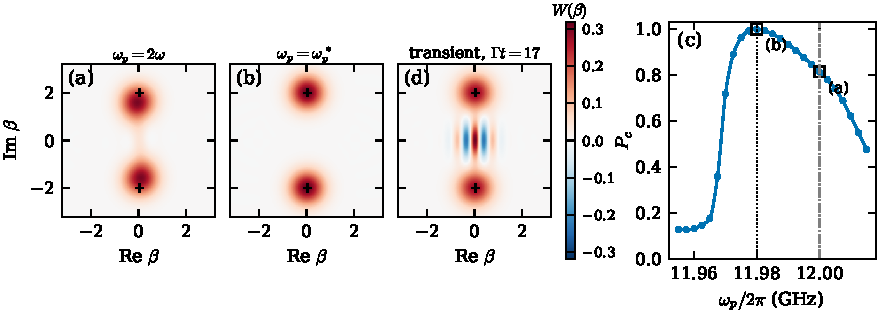
\includegraphics[width=\textwidth]{fig2_wigner.pdf}
\caption{Funciones de Wigner del oscilador (qubit trazado) en el esquema de Ma et al. (a) Estado estacionario con $\omega_{p}=2\omega$: amplitud reducida ($\alpha_{\rm eff}^{2}\approx-2.5$) y peso fuera del c\'odigo. (b) Estado estacionario con $\omega_{p}=\omega_{p}^{*}$: dos l\'obulos en $\pm2i$ sin franjas, porque en el estado estacionario la paridad ya decay\'o. (d) Transitorio en $\Gamma t=17$ con franjas de interferencia (gato par). (c) $P_{c}(\omega_{p})$.}
\end{figure}

%======================================================================
\section{Eliminaci\'on del qubit: tasas de uno y dos fonones}
\label{sec:RS}

\subsection{Formalismo de operadores efectivos}

Para un sistema con subespacio fundamental y subespacio excitado acoplados por perturbaciones $V_{+}$ (excita) y $V_{-}=V_{+}^{\dagger}$, con el subespacio excitado decayendo por $L$, el formalismo de Reiter y S{\o}rensen \cite{ReiterSorensen2012} da
\begin{equation}
L_{\rm ef}=L\,H_{\rm NH}^{-1}V_{+},\qquad H_{\rm ef}=-\frac{1}{2}V_{-}\left[H_{\rm NH}^{-1}+\left(H_{\rm NH}^{-1}\right)^{\dagger}\right]V_{+},
\end{equation}
con $H_{\rm NH}=H_{e}-\tfrac{i}{2}L^{\dagger}L$ el Hamiltoniano no herm\'itico del subespacio excitado. Para cada proceso con desinton\'ia $\Delta$ del estado intermedio, $H_{\rm NH}=\Delta-i\kappa/2$ y
\begin{equation}
H_{\rm NH}^{-1}=\frac{\Delta+i\kappa/2}{\Delta^{2}+\kappa^{2}/4},\qquad H_{\rm NH}^{-1}+(H_{\rm NH}^{-1})^{\dagger}=\frac{2\Delta}{\Delta^{2}+\kappa^{2}/4}.
\end{equation}

\subsection{Disipaci\'on de pares}

En el marco del drive y en la resonancia, el proceso $\ket{g}\to\ket{e}$ con $V_{+}=(-Ga^{2}+\Omega)\spl$ tiene $\Delta=0$. Entonces
\begin{equation}
L_{2}=\sqrt\kappa\,\smi\left(\frac{2i}{\kappa}\right)(-Ga^{2}+\Omega)\spl=-\frac{2iG}{\sqrt\kappa}\left(a^{2}-\alpha^{2}\right),\qquad H_{\rm ef}=0,
\end{equation}
proyectado sobre $\ket{g}$. La din\'amica efectiva es $\kappa_{2}\D[a^{2}-\alpha^{2}]$ con
\begin{equation}
\boxed{\kappa_{2}=\frac{4G^{2}}{\kappa}=\frac{16g_{x}^{2}g_{z}^{2}}{\omega^{2}\kappa}}.
\end{equation}
Se desprecian aqu\'i los corrimientos del qubit dependientes de $n$, que dan correcciones de orden superior.

\subsection{P\'erdida y ganancia de un fon\'on}

El t\'ermino rotante $V_{+}=g_{x}a\spl$ conecta $\ket{g,n}$ con $\ket{e,n-1}$, desintonizado en $\Delta_{1}=\omega_{q}-\omega\approx\omega$. El contrarrotante $V_{+}=g_{x}a^{\dagger}\spl$ conecta con $\ket{e,n+1}$, desintonizado en $\Delta_{3}=\omega_{q}+\omega\approx3\omega$. Para el primero,
\begin{equation}
L_{1}^{-}=\sqrt\kappa\,\smi\frac{g_{x}a\spl}{\Delta_{1}-i\kappa/2},\qquad \Gamma_{1}^{-}=\frac{g_{x}^{2}\kappa}{\Delta_{1}^{2}+\kappa^{2}/4},
\end{equation}
con disipador $\Gamma_{1}^{-}\D[a]$; y an\'alogamente
\begin{equation}
\Gamma_{1}^{+}=\frac{g_{x}^{2}\kappa}{\Delta_{3}^{2}+\kappa^{2}/4},
\end{equation}
con disipador $\Gamma_{1}^{+}\D[a^{\dagger}]$. Con $\kappa\ll\omega$,
\begin{equation}
\boxed{\Gamma_{1}^{-}\simeq\frac{g_{x}^{2}\kappa}{\omega^{2}},\qquad \Gamma_{1}^{+}\simeq\frac{g_{x}^{2}\kappa}{9\omega^{2}},\qquad \kappa_{1}\equiv\Gamma_{1}^{-}+\Gamma_{1}^{+}=\frac{10}{9}\frac{g_{x}^{2}\kappa}{\omega^{2}}}.
\end{equation}
Es el efecto Purcell del oscilador a trav\'es del qubit desintonizado, con su contraparte contrarrotante.

\subsection{Consistencia con el corrimiento}

El Hamiltoniano efectivo del mismo formalismo da, para el proceso rotante, $H_{\rm ef}=-\tfrac12 V_{-}[\ldots]V_{+}=-g_{x}^{2}\Delta_{1}a^{\dagger}a\,\Pg/(\Delta_{1}^{2}+\kappa^{2}/4)$, y para el contrarrotante $-g_{x}^{2}\Delta_{3}aa^{\dagger}\Pg/(\Delta_{3}^{2}+\kappa^{2}/4)$. En el l\'imite $\kappa\to0$ la suma es $-(g_{x}^{2}/\omega)n-(g_{x}^{2}/3\omega)(n+1)$, id\'entica a la parte en $\ket{g}$ de la Ec.~\eqref{eq:Hef}. Con $\kappa$ finito, el coeficiente de $n$ es
\begin{equation}
\delta_{1}=-g_{x}^{2}\left[\frac{\omega}{\omega^{2}+\kappa^{2}/4}+\frac{3\omega}{9\omega^{2}+\kappa^{2}/4}\right].
\end{equation}
Expandiendo con $x=\kappa/2$: $\omega/(\omega^{2}+x^{2})\approx(1/\omega)(1-x^{2}/\omega^{2})$ y $3\omega/(9\omega^{2}+x^{2})\approx(1/3\omega)(1-x^{2}/9\omega^{2})$, as\'i que
\begin{equation}
\delta_{1}\approx-\frac{4g_{x}^{2}}{3\omega}+\frac{g_{x}^{2}x^{2}}{\omega^{3}}\left(1+\frac{1}{27}\right)=-\frac{4g_{x}^{2}}{3\omega}\left[1-\frac{7}{9}\left(\frac{\kappa}{2\omega}\right)^{2}\right].
\end{equation}
La Tarea 41 lo confirma a cuatro cifras: el $\delta_{1}$ de Naseem es $\delta_{\rm osc}$ con esta correcci\'on.

%======================================================================
\section{Tasa de phase-flip}
\label{sec:pf}

\subsection{Evoluci\'on de la paridad}

Sea $P=e^{i\pi n}$. Como $Pa=-aP$ y $Pa^{\dagger}=-a^{\dagger}P$, el disipador adjunto sobre $P$ vale
\begin{align}
\D^{\dagger}[a]P&=a^{\dagger}Pa-\tfrac12\{n,P\}=-nP-nP=-2nP,\\
\D^{\dagger}[a^{\dagger}]P&=aPa^{\dagger}-\tfrac12\{aa^{\dagger},P\}=-(n+1)P-(n+1)P=-2(n+1)P.
\end{align}
Los t\'erminos de pares conmutan con $P$. Por tanto
\begin{equation}
\frac{d\langle P\rangle}{dt}=-2\Gamma_{1}^{-}\langle nP\rangle-2\Gamma_{1}^{+}\langle(n+1)P\rangle.
\end{equation}
En el espacio del c\'odigo, $\langle nP\rangle\simeq|\alpha|^{2}\langle P\rangle$, de donde
\begin{equation}
\boxed{\gamma_{\rm pf}=2\left[\Gamma_{1}^{-}|\alpha|^{2}+\Gamma_{1}^{+}\left(|\alpha|^{2}+1\right)\right]}.
\end{equation}
El $+1$ proviene de que la ganancia act\'ua sobre $\langle n+1\rangle$. Respecto a la forma aproximada $2|\alpha|^{2}\kappa_{1}$, la correcci\'on relativa es $\Gamma_{1}^{+}/(\kappa_{1}|\alpha|^{2})\approx1/(10|\alpha|^{2})$. Con p\'erdida intr\'inseca se agrega $\gamma$ a $\Gamma_{1}^{-}$.

\subsection{Piso de la paridad}

La paridad de un estado coherente es $\langle\alpha|P|\alpha\rangle=\langle\alpha|{-\alpha}\rangle=e^{-2|\alpha|^{2}}$. El estado estacionario, mezcla de $\ket{\pm\alpha}$, tiene entonces paridad $e^{-2|\alpha|^{2}}\approx3.4\times10^{-4}$ para $|\alpha|^{2}=4$. Por eso los ajustes de la tasa usan $A e^{-\gamma_{\rm pf}t}+c$.

\subsection{Verificaci\'on}

\begin{table}[h]
\centering
\begin{tabular}{lccc}
\toprule
medida & tasa & predicci\'on & raz\'on\\
\midrule
Ma, $\omega_{p}^{*}$, ajuste logar\'itmico $\Gamma t\in[26,152]$ (trabajo / V3) & $3.309/3.307\times10^{-4}$ & $3.333\times10^{-4}$ (sin $+1$) & 0.992\\
Ma, ajuste con piso (V3) & $3.332\times10^{-4}$ & $3.333\times10^{-4}$ (sin $+1$) & 1.000\\
Ma, con piso, f\'ormula con $+1$ y $|\langle a^{2}\rangle|=3.973$ & $3.332\times10^{-4}$ & $3.394\times10^{-4}$ & 0.982\\
\bottomrule
\end{tabular}
\caption{El acuerdo de 1.000 con la f\'ormula sin $+1$ fue una compensaci\'on: el $+1$ agrega 2.5\% y el r\'egimen saturado de Ma ($\kappa_{2}/\kappa=1$) resta $\sim2\%$.}
\end{table}

\begin{center}
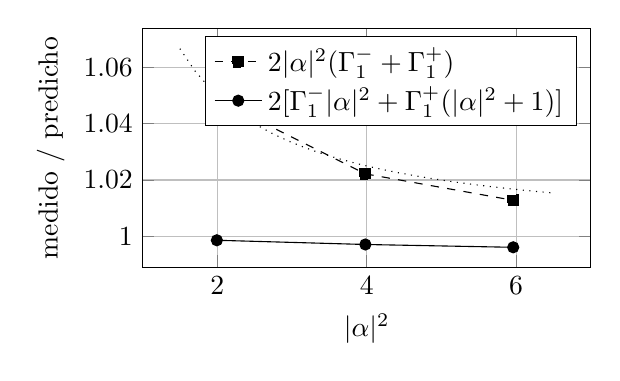
\begin{tikzpicture}
\begin{axis}[width=0.6\textwidth,height=0.38\textwidth,xlabel={$|\alpha|^{2}$},ylabel={medido / predicho},legend pos=north east,legend cell align=left,grid=major]
\addplot[mark=square*,dashed] coordinates {(1.9945,1.0486)(3.9819,1.0222)(5.9607,1.0128)};
\addlegendentry{$2|\alpha|^{2}(\Gamma_{1}^{-}+\Gamma_{1}^{+})$}
\addplot[mark=*] coordinates {(1.9945,0.9986)(3.9819,0.9971)(5.9607,0.9961)};
\addlegendentry{$2[\Gamma_{1}^{-}|\alpha|^{2}+\Gamma_{1}^{+}(|\alpha|^{2}+1)]$}
\addplot[dotted,domain=1.5:6.5] {1+1/(10*x)};
\end{axis}
\end{tikzpicture}
\end{center}
Verificaci\'on V4b en $(g_{x},\omega,g_{z}/\kappa)=(0.05,6,4)$ con $|\alpha|^{2}=|\langle a^{2}\rangle|$: la f\'ormula con $+1$ queda al 0.4\%. La l\'inea punteada es $1+1/(10|\alpha|^{2})$.

%======================================================================
\section{Figura de m\'erito}

\subsection{Derivaci\'on}

Dividiendo $\kappa_{1}$ entre $\kappa_{2}$:
\begin{equation}
\frac{\kappa_{1}}{\kappa_{2}}=\frac{10}{9}\frac{g_{x}^{2}\kappa}{\omega^{2}}\cdot\frac{\omega^{2}\kappa}{16g_{x}^{2}g_{z}^{2}}=\frac{10}{144}\frac{\kappa^{2}}{g_{z}^{2}},
\end{equation}
\begin{equation}
\boxed{\frac{\kappa_{1}}{\kappa_{2}}=\frac{5}{72}\left(\frac{\kappa}{g_{z}}\right)^{2}}.
\end{equation}
Se cancelan $g_{x}$ y $\omega$: el mismo acoplamiento transversal abre ambos canales con la misma dependencia $g_{x}^{2}/\omega^{2}$. Solo $g_{z}$ distingue los procesos, y $\kappa$ entra en el numerador de uno y el denominador del otro.

\subsection{Consecuencias de dise\~no}

\begin{enumerate}
\item Aumentar $g_{x}$ acelera el esquema pero no mejora la calidad; la calidad la fija $g_{z}/\kappa$.
\item El umbral del c\'odigo de repetici\'on, $\kappa_{2}/\kappa_{1}=220$ \cite{GuillaudMirrahimi2021}, exige $g_{z}/\kappa\geq\sqrt{(5/72)\cdot220}=3.9$ solo por este canal; para $\kappa_{1}/\kappa_{2}=10^{-3}$, $g_{z}/\kappa\geq8.3$.
\item El cociente empeora como $\kappa^{2}$ al aumentar la p\'erdida del qubit. Esto contradice la receta de Naseem \cite{Naseem2026}, que propone elegir $\kappa$ grande para suprimir los canales de un fon\'on frente a $\Gamma_{2}^{-}$.
\end{enumerate}

\subsection{Verificaci\'on}

\begin{table}[h]
\centering
\begin{tabular}{cccccc}
\toprule
$g_{x}$ & $\omega$ & $g_{z}/\kappa$ & $\kappa_{2}/\kappa$ & raz\'on (f\'ormula sin $+1$, $|\alpha|^{2}=4$) & raz\'on (con $+1$, $|\langle a^{2}\rangle|$)\\
\midrule
0.03 & 6 & 4 & 0.006 & 1.018 & 0.998\\
0.05 & 5 & 4 & 0.026 & 1.015 & 0.996\\
0.1 & 7 & 4 & 0.052 & 1.018 & 0.996\\
0.15 & 6 & 4 & 0.160 & 1.016 & 0.990\\
0.05 & 6 & 5 & 0.028 & 1.014 & 0.996\\
0.12 & 7 & 7 & 0.230 & 1.009 & 0.993\\
0.05 & 7 & 10 & 0.082 & 0.998 & 0.992\\
0.08 & 5 & 10 & 0.410 & 0.973 & 0.984\\
0.1 & 4 & 10 & 1.000 & 0.947 & 0.977\\
0.05 & 6 & 12 & 0.160 & 0.975 & 0.986\\
\bottomrule
\end{tabular}
\caption{Verificaci\'on independiente (V4 y V4b), modelo completo en el laboratorio, m\'etodo espectral. A $g_{z}/\kappa=4$ la raz\'on no depende de $g_{x}$ ni de $\omega$ (dispersi\'on 0.3\%).}
\end{table}

La precisi\'on depende de $\kappa_{2}/\kappa$, no de $g_{z}/\kappa$: $\lesssim0.4\%$ para $\kappa_{2}/\kappa\lesssim0.05$, $\sim1\%$ en $0.2$ y $\sim2\%$ en $1$. La f\'ormula es el resultado de orden dominante, exacto cuando $\kappa_{2}/\kappa\to0$; el d\'eficit es la primera correcci\'on no adiab\'atica. En $\kappa/g_{z}=0.1$ hay tres puntos con igual $g_{z}/\kappa$ y distinto $\kappa_{2}/\kappa$ cuya raz\'on baja con $\kappa_{2}/\kappa$ (0.992, 0.985 y 0.979).

\begin{figure}[h]
\centering
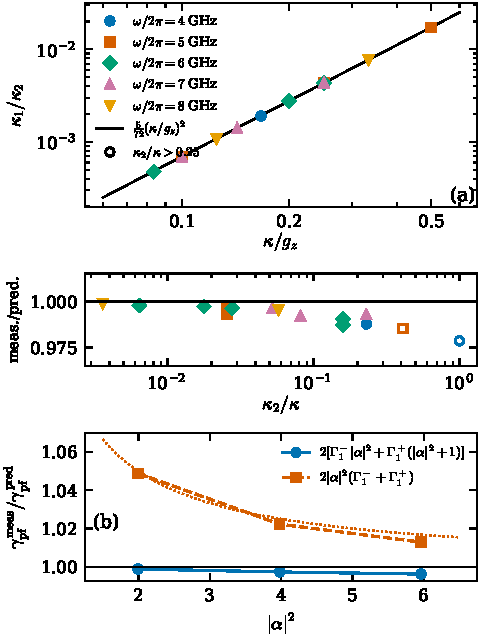
\includegraphics[width=0.62\textwidth]{fig3_val.pdf}
\caption{(a) $\kappa_{1}/\kappa_{2}$ frente a $\kappa/g_{z}$ para 15 puntos con $\omega/2\pi$ entre 4 y 8 GHz; relleno si $\kappa_{2}/\kappa\leq0.25$. Subpanel: cociente medido/predicho. (b) Cociente de la tasa de phase-flip medida y predicha frente a $|\alpha|^{2}$, con y sin el $+1$.}
\end{figure}

%======================================================================
\section{Baño estructurado del qubit}

\subsection{Autoenerg\'ia y tasas filtradas}

Si el qubit decae a trav\'es de un modo filtro de frecuencia $\omega_{f}=2\omega$, ancho $\kappa_{f}$ y acoplamiento $J(\spl b+\smi b^{\dagger})$, su autoenerg\'ia a energ\'ia $E$ es
\begin{equation}
\Sigma(E)=\frac{J^{2}}{E-\omega_{f}+i\kappa_{f}/2},\qquad \kappa_{\rm eff}(\delta)=-2\,{\rm Im}\,\Sigma=\frac{4J^{2}\kappa_{f}}{4\delta^{2}+\kappa_{f}^{2}},
\end{equation}
con $\delta=E-\omega_{f}$. Se fija $4J^{2}/\kappa_{f}=\kappa$, de modo que $\kappa_{\rm eff}(0)=\kappa$ y
\begin{equation}
\kappa_{\rm eff}(\delta)=\frac{\kappa\,\kappa_{f}^{2}}{4\delta^{2}+\kappa_{f}^{2}}.
\end{equation}
En cada proceso de la Secci\'on~\ref{sec:RS} el estado intermedio est\'a desintonizado en $\Delta$ respecto al estado inicial, y la autoenerg\'ia se eval\'ua a esa energ\'ia, lo que corresponde a $\delta=\Delta$ respecto al filtro. El proceso de pares es resonante con el filtro ($\delta=0$), el de p\'erdida tiene $\delta=\omega$ y el de ganancia $\delta=3\omega$:
\begin{equation}
\kappa_{2}=\frac{4G^{2}}{\kappa(0)},\qquad \Gamma_{1}^{-}=\frac{g_{x}^{2}\kappa_{\rm eff}(\omega)}{\omega^{2}},\qquad \Gamma_{1}^{+}=\frac{g_{x}^{2}\kappa_{\rm eff}(3\omega)}{9\omega^{2}},
\end{equation}
y la figura de m\'erito generalizada es
\begin{equation}
\boxed{\frac{\kappa_{1}}{\kappa_{2}}=\frac{\kappa(0)\left[\kappa_{\rm eff}(\omega)+\kappa_{\rm eff}(3\omega)/9\right]}{16g_{z}^{2}}},
\end{equation}
que para baño plano se reduce a $(5/72)(\kappa/g_{z})^{2}$. Para $\kappa_{f}\ll\omega$, la mejora sobre el canal de p\'erdida es $\kappa/\kappa_{\rm eff}(\omega)=(4\omega^{2}+\kappa_{f}^{2})/\kappa_{f}^{2}\approx4\omega^{2}/\kappa_{f}^{2}$.

\subsection{Verificaci\'on}

\begin{table}[h]
\centering
\begin{tabular}{ccccc}
\toprule
baño & $\Gamma_{1}^{-}$ medido/predicho & $\Gamma_{1}^{+}$ medido/predicho & mejora de $\gamma_{\rm pf}$ medida & predicha (con $+1$)\\
\midrule
plano & 1.0004 & 0.9995 & 1 & 1\\
$\kappa_{f}=3$ & -- & -- & 19.5 & --\\
$\kappa_{f}=1$ & 0.9980 & 1.0011 & 166.5 & 166.1\\
$\kappa_{f}=0.3$ & 0.9977 & 1.0011 & 1838 & 1833\\
$\kappa_{f}=0.1$ & -- & -- & $1.65\times10^{4}$ & --\\
\bottomrule
\end{tabular}
\caption{Par\'ametros de Ma, $|\alpha|^{2}=2$. Canales separados por el Liouvilliano est\'atico sin drive (V5); mejoras por la tasa del modo de paridad con drive (Tarea 43 y V5). Comparar con $\kappa_{1}$ en lugar de $\gamma_{\rm pf}$ subestima la mejora un 4\% porque el filtro suprime $\Gamma_{1}^{+}$ m\'as que $\Gamma_{1}^{-}$.}
\end{table}

\begin{center}
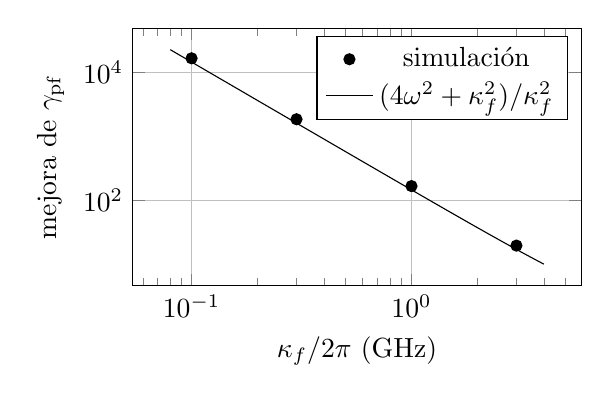
\begin{tikzpicture}
\begin{axis}[width=0.6\textwidth,height=0.4\textwidth,xmode=log,ymode=log,xlabel={$\kappa_{f}/2\pi$ (GHz)},ylabel={mejora de $\gamma_{\rm pf}$},grid=major,legend pos=north east]
\addplot[only marks,mark=*] coordinates {(3,19.5)(1,166)(0.3,1840)(0.1,16500)};
\addlegendentry{simulaci\'on}
\addplot[domain=0.08:4,samples=60] {(4*36+x^2)/x^2};
\addlegendentry{$(4\omega^{2}+\kappa_{f}^{2})/\kappa_{f}^{2}$}
\end{axis}
\end{tikzpicture}
\end{center}

El costo es la tasa de confinamiento, que cae de $4.2\times10^{-3}$ (plano) a $3.6$, $3.1$, $2.2$ y $0.98\times10^{-3}$ para $\kappa_{f}=3,1,0.3,0.1$, porque con filtros estrechos el baño deja de ser markoviano. Este costo no est\'a convergido en $N$ (6\%) y es cualitativo. El filtro arm\'onico ($N_{f}=3,4$) y el de dos niveles difieren en menos del 3\%.

%======================================================================
\section{Confinamiento con un auxiliar de dos niveles}

\subsection{Modelo m\'inimo}

$H=G[(a^{2}-\alpha^{2})\spl+{\rm h.c.}]$, con $\kappa\D[\smi]$ y $\Gamma_{2}\equiv4G^{2}/\kappa$. La ecuaci\'on maestra se reescribe como
\begin{equation}
\Lv\rho=-i(H_{\rm NH}\rho-\rho H_{\rm NH}^{\dagger})+\kappa\smi\rho\spl,\qquad H_{\rm NH}=H-\frac{i\kappa}{2}\spl\smi.
\end{equation}

\subsection{Soluci\'on exacta para $\alpha=0$}

\paragraph{Cantidad conservada.} $\hat N=n+2\spl\smi$ conmuta con $H$: $[n,a^{2}]=-2a^{2}$ y $[2\spl\smi,\spl]=2\spl$ dan $[\hat N,a^{2}\spl]=-2a^{2}\spl+2a^{2}\spl=0$, y lo mismo para el herm\'itico conjugado.

\paragraph{Bloques.} Los autoestados de $\hat N$ son $\ket{0,g}$ ($N=0$), $\ket{1,g}$ ($N=1$) y los pares $\{\ket{N,g},\ket{N-2,e}\}$ ($N\geq2$), con elemento $G_{N}=G\sqrt{N(N-1)}$:
\begin{equation}
H_{N}=\begin{pmatrix}0&G_{N}\\G_{N}&-i\kappa/2\end{pmatrix},\qquad E_{N,\pm}=-\frac{i\kappa}{4}\pm\sqrt{G_{N}^{2}-\frac{\kappa^{2}}{16}}.
\end{equation}
El salto lleva el sector $(N,M)$ al $(N-2,M-2)$, as\'i que $\Lv$ es triangular por bloques y sus autovalores son $\lambda=-i(E_{i}^{(N)}-E_{j}^{(M)*})$.

\paragraph{Modo m\'as lento.} Es la coherencia entre el espacio oscuro ($E=0$) y el bloque $N=2$, con tasa $\kappa/4-\delta_{2}$, $\delta_{2}=\sqrt{\kappa^{2}/16-2G^{2}}=(\kappa/4)\sqrt{1-8\Gamma_{2}/\kappa}$. Resultado:
\begin{equation}
\boxed{\Delta=\begin{cases}\dfrac{\kappa}{4}\left[1-\sqrt{1-\dfrac{8\Gamma_{2}}{\kappa}}\right],&\Gamma_{2}\leq\kappa/8,\\[2ex]\dfrac{\kappa}{4},&\Gamma_{2}\geq\kappa/8,\end{cases}}
\end{equation}
con un punto excepcional en $\Gamma_{2}=\kappa/8$. L\'imite adiab\'atico: $\Delta\approx\Gamma_{2}+2\Gamma_{2}^{2}/\kappa$. Verificado a precisi\'on de m\'aquina en 18 valores (V6).

\subsection{Techo $\kappa/4$ para $\alpha\neq0$}

Para un autovector derecho $\ket{r}$ de $H_{\rm NH}$ con autovalor $E$, $E\langle r|r\rangle=\langle r|H|r\rangle-(i\kappa/2)\langle r|\spl\smi|r\rangle$, y como $H$ es herm\'itico,
\begin{equation}
{\rm Im}\,E=-\frac{\kappa}{2}p_{e}(r),\qquad p_{e}(r)=\frac{\langle r|\spl\smi|r\rangle}{\langle r|r\rangle}.
\end{equation}
En acoplamiento fuerte los estados vestidos tienen $p_{e}\to1/2$, y la coherencia con el espacio oscuro decae a $\kappa/4$. Para $\alpha\neq0$ el argumento es aproximado; la num\'erica lo confirma.

\begin{center}
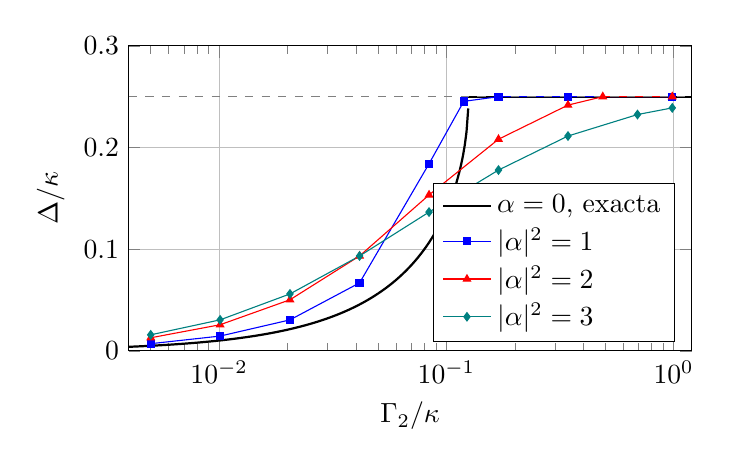
\begin{tikzpicture}
\begin{axis}[width=0.72\textwidth,height=0.45\textwidth,xmode=log,xmin=0.004,xmax=1.2,ymin=0,ymax=0.3,xlabel={$\Gamma_{2}/\kappa$},ylabel={$\Delta/\kappa$},legend pos=south east,legend cell align=left,grid=major]
\addplot[black,thick,domain=0.004:0.125,samples=200] {0.25*(1-sqrt(1-8*x))};
\addlegendentry{$\alpha=0$, exacta}
\addplot[black,thick,forget plot,domain=0.125:1.2] {0.25};
\addplot[blue,mark=square*,mark size=1.3pt] coordinates {(0.0050,0.00711)(0.0101,0.01459)(0.0205,0.03051)(0.0415,0.06690)(0.0839,0.18404)(0.1193,0.24538)(0.1696,0.25)(0.3430,0.25)(0.9865,0.25)};
\addlegendentry{$|\alpha|^{2}=1$}
\addplot[red,mark=triangle*,mark size=1.5pt] coordinates {(0.0050,0.01292)(0.0101,0.02574)(0.0205,0.05029)(0.0415,0.09338)(0.0839,0.15335)(0.1696,0.20815)(0.3430,0.24171)(0.4878,0.25)(0.9865,0.25)};
\addlegendentry{$|\alpha|^{2}=2$}
\addplot[teal,mark=diamond*,mark size=1.5pt] coordinates {(0.0050,0.01583)(0.0101,0.03055)(0.0205,0.05603)(0.0415,0.09335)(0.0839,0.13651)(0.1696,0.17783)(0.3430,0.21130)(0.6937,0.23242)(0.9865,0.23897)};
\addlegendentry{$|\alpha|^{2}=3$}
\addplot[gray,dashed,domain=0.004:1.2] {0.25};
\end{axis}
\end{tikzpicture}
\end{center}

\subsection{Modelo completo}

En el modelo completo de Naseem, el espectro de Floquet contiene modos de borde del truncamiento (con $|{\rm Im}\lambda|\propto N$) y una rama interior no convergida para $\Gamma_{2}/\kappa\gtrsim0.25$. La tasa de confinamiento din\'amicamente relevante, medida por el regreso al c\'odigo desde tres estados iniciales, es 0.175, 0.23 y 0.26--0.29 en $\Gamma_{2}/\kappa=0.13$, 0.3 y 1, y coincide con el modelo est\'atico con buffer expl\'icito (0.234 en $\Gamma_{2}/\kappa=1$). El peso de los estados f\'isicos sobre la rama no convergida es de $10^{-16}$ a $10^{-13}$. El m\'aximo de la brecha en $\Gamma_{2}/\kappa\approx0.13$ reportado en tareas tempranas era un artefacto de esos modos.

%======================================================================
\section{Base polar\'onica del c\'odigo}
\label{sec:polaron}

Con el qubit en $\ket{g}$, la parte del oscilador de la Ec.~\eqref{eq:H} es $\omega n-g_{z}(a+a^{\dagger})$. Completando el cuadrado,
\begin{equation}
\omega a^{\dagger}a-g_{z}(a+a^{\dagger})=\omega\left(a-\frac{g_{z}}{\omega}\right)^{\dagger}\left(a-\frac{g_{z}}{\omega}\right)-\frac{g_{z}^{2}}{\omega},
\end{equation}
as\'i que el oscilador est\'a desplazado en $d=+g_{z}/\omega$ en el marco de laboratorio. En los instantes estrobosc\'opicos $t=nT_{p}$ el c\'odigo es $\{D(g_{z}/\omega)\ket{\pm\alpha}\}$; en el marco que rota a $\omega_{p}/2$ el desplazamiento aparecer\'ia con signo alternante.

Decisiones: $P_{c}$ y todas las curvas de confinamiento usan el c\'odigo fijo $\{D(g_{z}/\omega)\ket{\pm\alpha_{\rm nom}}\}$ con $\alpha_{\rm nom}^{2}=\Omega/G$. El valor medido $\alpha_{\rm eff}^{2}=\langle(a-d)^{2}\rangle$ se usa solo en la tasa de phase-flip. Un c\'odigo adaptado al estado no sirve para $P_{c}$: lejos de la resonancia seguir\'ia al estado encogido y dar\'ia $P_{c}$ alto (0.967 en $\omega_{p}=12$ con $\alpha_{\rm eff}^{2}=-2.48$).

Efecto: en la resonancia de Ma, $1-P_{c}$ baja de $2.5\times10^{-3}$ a $1.3\times10^{-3}$; en $(g_{x},\omega,g_{z}/\kappa)=(0.05,6,12)$, de $5.0\times10^{-3}$ a $1.3\times10^{-3}$. La ca\'ida de $P_{c}$ al aumentar $g_{z}$ era casi toda un efecto de base: la deficiencia escala como $(g_{z}/\omega)^{2}$.

%======================================================================
\section{Temperatura}
\label{sec:termico}

Con el qubit a temperatura $T$, $n_{q}=[\exp(hf_{q}/k_{B}T)-1]^{-1}$, y la din\'amica incluye $\kappa(n_{q}+1)\D[\smi]+\kappa n_{q}\D[\spl]$. Cada excitaci\'on t\'ermica del qubit puede producir un bit-flip. En el esquema de Naseem ($\Gamma_{2}/\kappa=0.13$), $\gamma_{\rm bf}\approx0.05n_{q}\kappa$, y el sesgo $\eta=\gamma_{\rm pf}/\gamma_{\rm bf}$ depende solo de $x=hf_{q}/k_{B}T$:

\begin{center}
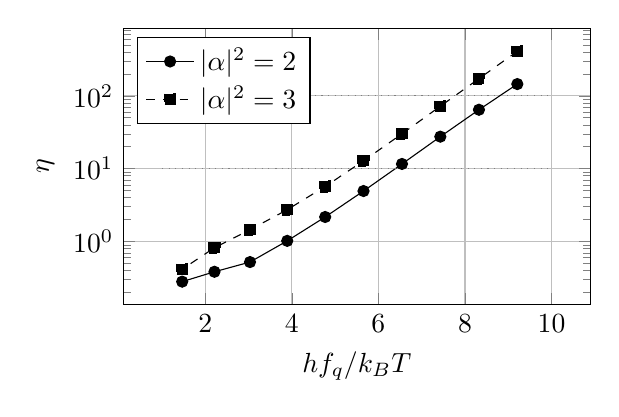
\begin{tikzpicture}
\begin{axis}[width=0.62\textwidth,height=0.42\textwidth,ymode=log,xlabel={$hf_{q}/k_{B}T$},ylabel={$\eta$},legend pos=north west,grid=major]
\addplot[mark=*] coordinates {(9.21,145)(8.323,64.4)(7.431,27.5)(6.545,11.6)(5.656,4.93)(4.77,2.17)(3.893,1.02)(3.033,0.522)(2.212,0.384)(1.466,0.281)};
\addlegendentry{$|\alpha|^{2}=2$}
\addplot[mark=square*,dashed] coordinates {(9.21,409)(8.323,172)(7.431,72)(6.545,30.1)(5.656,12.8)(4.77,5.69)(3.893,2.73)(3.033,1.45)(2.212,0.821)(1.466,0.416)};
\addlegendentry{$|\alpha|^{2}=3$}
\addplot[gray,dotted,domain=1:10] {100};
\addplot[gray,dotted,domain=1:10] {10};
\end{axis}
\end{tikzpicture}
\end{center}

Umbrales: sesgo 100 con $hf_{q}/k_{B}T=8.8$ ($|\alpha|^{2}=2$) y 7.8 ($|\alpha|^{2}=3$); sesgo 10 con 6.4 y 5.4. A 10 mK, un sesgo de 100 exige $f_{q}\gtrsim1.8$ GHz. Estos umbrales se calcularon en el r\'egimen de Naseem; seg\'un la Tarea 44, para $g_{2}/\kappa\lesssim0.1$ la supresi\'on exponencial en $|\alpha|^{2}$ se mantiene con un factor constante, en acuerdo con Gautier et al.\ \cite{Gautier2022}, y para $g_{2}/\kappa\gtrsim1$ cada excitaci\'on t\'ermica produce un bit-flip con probabilidad de orden uno. La limitaci\'on t\'ermica de los buffers a $2\omega$ es conocida para buffers arm\'onicos \cite{Marquet2024}.

%======================================================================
\section{Mapa de plataformas}

\begin{table}[h]
\centering
\begin{tabular}{lccc}
\toprule
 & Ma et al. & Naseem & Liu et al.\\
\midrule
$\kappa/\omega$ & 0.005 & 0.001 & 0.90\\
$g_{z}/\kappa$ & 7.1 & 60 & 0.22\\
$\kappa_{2}/\kappa$ & 1.0 & 2.07 & 0.031\\
$\kappa_{1}/\kappa_{2}$ & $1.4\times10^{-3}$ & $9.2\times10^{-5}$ & fuera de validez\\
$\kappa_{1}$/confinamiento medido & $1.0\times10^{-2}$ & $8.3\times10^{-4}$ & --\\
$hf_{q}/k_{B}T$ (10 mK) & 58 & 0.96 & --\\
veredicto & confinamiento saturado & falla t\'ermica & fuera del r\'egimen perturbativo\\
\bottomrule
\end{tabular}
\end{table}

En Liu et al., la simulaci\'on de su Ec.~(9) con la convenci\'on $\alpha^{2}=\varepsilon_{p}/g_{\rm eff}$ (la que reproduce su Fig.~2 con su modelo efectivo) no forma el gato: $F\leq0.35$ y $|\langle a^{2}\rangle|$ llega a la mitad del valor anal\'itico. Se reporta como caso fuera del r\'egimen perturbativo, sin extraer conclusiones sobre su Hamiltoniano completo.

%======================================================================
\section{M\'etodos num\'ericos}

\paragraph{Propagador de Floquet.} Como $H(t)$ es peri\'odico con $T_{p}=2\pi/\omega_{p}$ en el laboratorio, se calcula el propagador del superoperador sobre un per\'iodo integrando la ecuaci\'on maestra (tolerancias $10^{-12}$ y $10^{-10}$). La implementaci\'on original us\'o el marco rotante con per\'iodo $4\pi/\omega_{p}$; la verificaci\'on independiente us\'o el laboratorio.

\paragraph{Muestreo estrobosc\'opico.} En $t=nT_{p}$, pasar al marco que rota a $\omega_{p}/2$ multiplica $a$ por $e^{-i\pi n}=(-1)^{n}$, lo que deja invariantes el espacio del c\'odigo, $\langle a^{2}\rangle$, $P_{e}$ y la paridad. $P_{e}$ y la paridad tienen micromovimiento dentro del per\'iodo; $P_{c}$ var\'ia menos de $3\times10^{-5}$.

\paragraph{M\'etodo espectral.} Las tasas son $r_{k}=-\ln|\lambda_{k}|/T_{p}$. El modo de paridad tiene $\lambda$ real cercano a $+1$ y el mayor $|{\rm Tr}(PR_{k})|/\|R_{k}\|$ (alrededor de 1.41, frente a menos de 0.05 en los dem\'as modos lentos).

\paragraph{Modos espurios.} Un modo es espurio si su peso de borde (norma con $n>N-6$) es mayor que 0.5 o si su autovalor no es estable al 0.3\% en tres truncamientos $N$, $N+6$, $N+12$. Los que no cumplen la estabilidad sin superar el peso de borde se reportan como no resueltos.

\paragraph{Validaciones.} En toda matriz densidad: $|{\rm Tr}\rho-1|<10^{-10}$, $\|\rho-\rho^{\dagger}\|<10^{-10}$ y m\'inimo autovalor mayor que $-10^{-9}$. Convergencia en $N$ en al menos un punto por resultado.

%======================================================================
\section{Verificaci\'on independiente}

Un segundo modelo (Opus), sin acceso al c\'odigo original, reimplement\'o los resultados centrales con formulaciones distintas.

\begin{table}[h]
\centering
\begin{tabular}{lll}
\toprule
& resultado & veredicto\\
\midrule
V1 & Hamiltoniano efectivo y corrimientos & confirma, a cuarto orden\\
V2 & resonancia vestida (laboratorio, sin RWA) & confirma; m\'aximo en 11.97993\\
V3 & tasa de paridad & confirma; ajuste con piso 1.000\\
V4 & figura de m\'erito, 8 puntos nuevos & confirma; independencia de $g_{x},\omega$ al 0.3\%\\
V4b & t\'ermino $+1$ y $|\alpha|^{2}$ efectivo & confirma; 0.4\%\\
V5 & baño filtrado, canal por canal & confirma; 0.2\%\\
V6 & brecha exacta & confirma a precisi\'on de m\'aquina\\
\bottomrule
\end{tabular}
\end{table}

%======================================================================
\section{Resultados corregidos o retirados}

\begin{enumerate}
\item El m\'aximo de la brecha en $\Gamma_{2}/\kappa\approx0.13$ y su saturaci\'on en 0.10--0.17$\kappa$: artefactos de modos de borde del truncamiento (Tareas 35, 38, 45 y 47).
\item La hip\'otesis de un punto excepcional como origen de ese m\'aximo: se sostiene solo para $\alpha=0$.
\item El umbral t\'ermico ``$hf_{q}/k_{B}T\gtrsim5$'': el valor correcto es 8.8 para sesgo 100 con $|\alpha|^{2}=2$; el 4.8 de la Tarea 37 est\'a en la frecuencia mec\'anica.
\item La precisi\'on ``$\leq0.4\%$ para $\kappa_{2}/\kappa\lesssim0.25$'': generalizaci\'on de un solo punto; la precisi\'on depende de $\kappa_{2}/\kappa$.
\item La tasa de phase-flip sin el $+1$ y el acuerdo de 1.000 en Ma: compensaci\'on de efectos.
\item El uso de $\alpha_{\rm eff}$ para $P_{c}$: descartado.
\item El signo del t\'ermino de pares expl\'icito en una variante de la Tarea 45(d): corregido antes de afectar otros resultados.
\end{enumerate}

%======================================================================
\section{Posicionamiento bibliogr\'afico}

\paragraph{Conocido.} El concepto de $\kappa_{1}/\kappa_{2}$ como figura de m\'erito \cite{GuillaudMirrahimi2021,Chamberland2022}; la calibraci\'on de frecuencias corridas por Stark en experimentos con buffer arm\'onico \cite{Putterman2025}; el efecto Purcell y los corrimientos dispersivos con Bloch-Siegert \cite{Zueco2009}; la p\'erdida de un fot\'on inducida por el mecanismo de estabilizaci\'on en circuitos con ATS \cite{Carde2024}; los canales de un fon\'on en la teor\'ia de Naseem \cite{Naseem2026}; la brecha con buffer arm\'onico \cite{Ferrari2026}; el buffer de dos niveles con p\'erdida y t\'ermico \cite{Gautier2022}; el an\'alogo arm\'onico directo (gato autoparam\'etrico) \cite{Marquet2024}; la estabilizaci\'on estrobosc\'opica con auxiliar de dos niveles \cite{Hillmann2026}.

\paragraph{No encontrado en ning\'un trabajo.} La expresi\'on $(5/72)(\kappa/g_{z})^{2}$, su independencia de $g_{x}$ y $\omega$, su versi\'on con baño estructurado y la dependencia correcta con $\kappa$. La revisi\'on de citas (Semantic Scholar: 14, 10, 12 y 0 citas de Ma, Liu, Hou y Naseem) no encontr\'o ning\'un trabajo que discuta la relaci\'on entre las tasas de uno y dos cuantos en esta familia.

\paragraph{Afirmaciones publicadas que se corrigen.} (i) La conservaci\'on de paridad en el estado estacionario (Ma, Liu, Hou y la revisi\'on \cite{Lu2026}): el estado estacionario es una mezcla. (ii) La receta de Naseem de aumentar $\kappa$: empeora el cociente como $\kappa^{2}$. (iii) La omisi\'on del corrimiento del oscilador en Ma, Liu y el c\'odigo de Naseem. (iv) El factor 2 en la Ec.~(11) de Naseem.

\paragraph{Alcance.} Vale para esquemas donde el intercambio de pares surge de combinar $g_{x}$ y $g_{z}$ a segundo orden, en el r\'egimen $\kappa,g\ll\omega$. No aplica al esquema de iones \cite{deMatos1996}, cuyo acoplamiento de pares es nativo.

%======================================================================
\section{Pendientes}

\begin{enumerate}
\item Figuras principales: colapso universal de la resonancia, mapa del espacio de dise\~no, mapa del baño, mapa t\'ermico con plataformas.
\item Explicaci\'on del d\'eficit no adiab\'atico de 1--2\% (posible correlaci\'on con $P_{e}$).
\item Tasa de confinamiento de Ma con $|\alpha|^{2}=4$.
\item Revisi\'on de citas en Google Scholar y lectura de Hou et al.
\item Propuesta de dise\~no concreta con par\'ametros reales de dispositivos de GHz.
\item Revisi\'on humana de las derivaciones y conversaci\'on sobre autor\'ia.
\end{enumerate}

\bibliographystyle{unsrt}
\bibliography{refs_doc}
\end{document}
